\documentclass[12pt]{article}
\usepackage[utf8]{inputenc}
\usepackage[spanish]{babel}
\spanishdecimal{.}
\usepackage{amsmath, amssymb}
\usepackage{array}
\usepackage{booktabs}
\usepackage{multirow}
\usepackage{graphicx}
\usepackage{grffile}
\usepackage{float}
\usepackage{geometry}
\usepackage{caption}
\usepackage{listings}
\usepackage{xcolor}
\geometry{margin=2.5cm}

\lstset{
  basicstyle=\ttfamily\footnotesize,
  breaklines=true,
  breakatwhitespace=false,
  columns=flexible,
  keepspaces=true,
  showstringspaces=false,
  frame=single,
  framesep=4pt,
  xleftmargin=8pt,
  xrightmargin=4pt,
  backgroundcolor=\color{gray!8},
  commentstyle=\color{gray!55},
  keywordstyle=\bfseries,
  extendedchars=true,
  inputencoding=utf8,
}

\title{Proyecto Final --- Regresi\'on Avanzada\\[6pt]
       \large An\'alisis Bayesiano Espacial de PM2.5 en el Valle de M\'exico}
\author{Paulina Garza Allende \and Andrea Monserrat Arredondo Rodr\'iguez}
\date{19 de mayo de 2026}

\begin{document}
\maketitle

%==============================================================
\section{Introducci\'on}
%==============================================================

El Valle de M\'exico es una cuenca hidrol\'ogica cerrada que alberga la
Zona Metropolitana del Valle de M\'exico (ZMVM), con aproximadamente
22~millones de habitantes.
Su geometr\'ia de cuenca cerrada impide la ventilaci\'on natural de los
contaminantes, lo que convierte al PM2.5 (material particulado fino con
di\'ametro aerodin\'amico $\leq 2.5\,\mu$m) en uno de los principales
problemas de salud p\'ublica de la regi\'on.
La exposici\'on cr\'onica a PM2.5 est\'a asociada con enfermedades
respiratorias, cardiovasculares y aumento en la mortalidad.

La fuente de datos es el Sistema Nacional de Informaci\'on de la
Calidad del Aire~(SINAICA), operado por el Instituto Nacional de
Ecolog\'ia y Cambio Clim\'atico.
Se descargaron datos de las 56 estaciones de monitoreo ubicadas dentro
de los l\'imites del Valle de M\'exico (16~alcald\'ias de la CDMX,
59~municipios del Estado de M\'exico, m\'as Tizayuca en Hidalgo).
De estas, solo 14~estaciones reportaron simult\'aneamente concentraci\'on
de PM2.5, temperatura y humedad relativa durante 2023,
con un total de 2{,}617~observaciones diarias (enero--septiembre de 2023).

La pregunta central de este proyecto es:
\begin{quote}
\emph{¿Qu\'e tan importante es la estructura espacial para explicar la variaci\'on
de PM2.5 en el Valle de M\'exico, y podemos usarla para predecir la
contaminaci\'on en zonas sin sensores?}
\end{quote}

Para responderla se comparan cinco modelos bayesianos de complejidad
creciente, ajustados con JAGS a trav\'es del paquete \texttt{R2jags}:

\begin{enumerate}
  \item \textbf{Modelo A --- Normal global}: ¿cu\'anto de la variaci\'on de PM2.5
        explican el clima y la estacionalidad, sin considerar la ubicaci\'on?
  \item \textbf{Modelo B --- Efectos fijos}: ¿existen diferencias sistem\'aticas
        entre estaciones que no se explican por clima?
  \item \textbf{Modelo C1 --- Jer\'arquico}: ¿es mejor modelar esas diferencias
        como un proceso aleatorio com\'un con encogimiento~(\emph{shrinkage})
        que como par\'ametros independientes?
  \item \textbf{Modelo C2 --- Gamma}: ¿es la distribuci\'on Gamma, que respeta
        el soporte positivo de PM2.5, mejor que la Normal sobre el logaritmo?
  \item \textbf{Modelo D --- Tendencia lat/lon}: ¿captura un gradiente lineal
        en latitud y longitud el patr\'on espacial, o se necesita un modelo
        no lineal?
\end{enumerate}

Finalmente, el \textbf{Modelo E} usa los efectos espaciales del Modelo~C1
para hacer kriging bayesiano y predecir PM2.5 en los 141~pol\'igonos del
Valle de M\'exico, incluyendo los 44~municipios de Edomex sin estaciones
de monitoreo.


%==============================================================
\section{Descripci\'on de la informaci\'on}
%==============================================================

\subsection*{Variables}

\begin{table}[H]
\centering
\caption{Variables utilizadas en el an\'alisis.}
\label{tab:variables}
\small
\begin{tabular}{>{\raggedright\arraybackslash}p{2.3cm}
                >{\raggedright\arraybackslash}p{6cm}
                >{\raggedright\arraybackslash}p{3.8cm}
                >{\raggedright\arraybackslash}p{2cm}}
\toprule
Variable & Descripci\'on & Rol & Escala \\
\midrule
\texttt{pm25}    & Concentraci\'on diaria promedio de PM2.5 ($\mu$g/m$^3$)
                 & Respuesta & Raz\'on \\
\texttt{temp}    & Temperatura diaria promedio (°C)
                 & Covariable meteorol\'ogica & Intervalo \\
\texttt{hr}      & Humedad relativa diaria promedio (\%)
                 & Covariable meteorol\'ogica & Intervalo \\
\texttt{sen\_t}  & $\sin(2\pi\cdot\text{d\'ia}/365)$
                 & Covariable estacional (Fourier) & Intervalo \\
\texttt{cos\_t}  & $\cos(2\pi\cdot\text{d\'ia}/365)$
                 & Covariable estacional (Fourier) & Intervalo \\
\texttt{lat, lon}& Coordenadas geogr\'aficas de la estaci\'on
                 & Predictor espacial & Intervalo \\
\texttt{estaci\'on}& Nombre de la estaci\'on de monitoreo
                 & Agrupador & Nominal \\
\bottomrule
\end{tabular}
\normalsize
\end{table}

La temperatura y la humedad relativa se estandarizaron
(media~0, desviaci\'on est\'andar~1) antes de ingresarlas a JAGS,
para mejorar la convergencia del MCMC y hacer comparables las magnitudes
de los coeficientes.
PM2.5 se transforma a escala logar\'itmica en todos los modelos
Normal~(A, B, C1, D), lo que estabiliza la varianza y linealiza la
relaci\'on con las covariables.

\subsection*{Estaciones de monitoreo}

\begin{table}[H]
\centering
\caption{Resumen por estaci\'on (datos 2023, n = 2{,}617 observaciones totales).}
\label{tab:estaciones}
\small
\begin{tabular}{>{\raggedright\arraybackslash}p{4.5cm}
                >{\raggedright\arraybackslash}p{2.8cm}rrrr}
\toprule
Estaci\'on & Municipio & n & Temp. & HR & PM2.5 \\
           &           &   & (°C) & (\%) & ($\mu$g/m$^3$) \\
\midrule
Santiago Acahualtepec & Iztapalapa       & 189 & 17.4 & 46.4 & 23.5 \\
Hospital General M\'exico & Cuauht\'emoc & 52  & 19.2 & 33.1 & 22.7 \\
Gustavo A. Madero      & G.~A.~Madero    & 154 & 19.4 & 45.2 & 22.7 \\
Tlalnepantla           & Tlalnepantla    & 174 & 18.5 & 41.9 & 21.8 \\
San Agust\'in          & Ecatepec        & 84  & 19.9 & 49.5 & 20.7 \\
UAM Iztapalapa         & Iztapalapa      & 207 & 19.7 & 49.5 & 20.6 \\
Merced                 & Venustiano C.   & 235 & 20.0 & 47.8 & 20.6 \\
UAM Xochimilco         & Coyoac\'an      & 233 & 17.5 & 48.2 & 20.5 \\
Nezahualc\'oyotl       & Nezahualc\'oyotl& 218 & 19.5 & 43.9 & 20.4 \\
Benito Ju\'arez        & Benito Ju\'arez & 236 & 19.2 & 45.3 & 19.8 \\
FES Arag\'on           & Nezahualc\'oyotl& 233 & 20.1 & 48.0 & 18.0 \\
Pedregal               & \'Alvaro Obreg\'on& 181& 17.2 & 49.7 & 16.2 \\
Ajusco Medio           & Tlalpan         & 188 & 14.5 & 55.2 & 16.0 \\
Biblioteca             & Tizayuca        & 233 & 14.5 & 50.9 & 15.4 \\
\bottomrule
\end{tabular}
\normalsize
\end{table}

El rango de concentraciones promedio entre estaciones va de
15.4~$\mu$g/m$^3$ (Biblioteca, Tizayuca) a
23.5~$\mu$g/m$^3$ (Santiago Acahualtepec, Iztapalapa),
una diferencia de 52\% entre la estaci\'on m\'as limpia y la m\'as
contaminada.
Todas las estaciones superan la gu\'ia de la OMS de 5~$\mu$g/m$^3$
para el promedio anual.

\subsection*{An\'alisis exploratorio}

\begin{figure}[H]
  \centering
  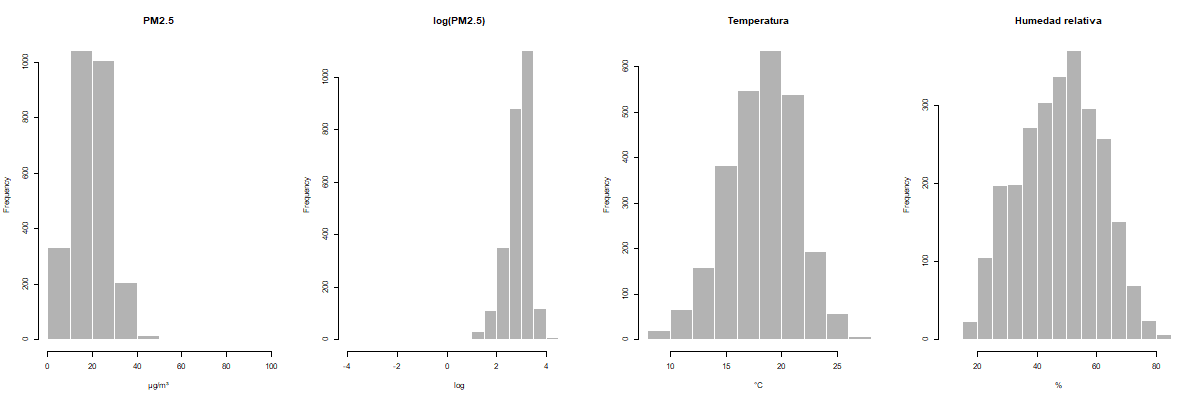
\includegraphics[width=\textwidth]{output/figures/eda_valle_v2_histogramas.png}
  \caption{Histogramas de las variables principales.
           La distribuci\'on de PM2.5 tiene cola derecha pronunciada;
           en escala logar\'itmica se aproxima m\'as a la Normal,
           lo que justifica la transformaci\'on utilizada en los modelos.}
\end{figure}

\begin{figure}[H]
  \centering
  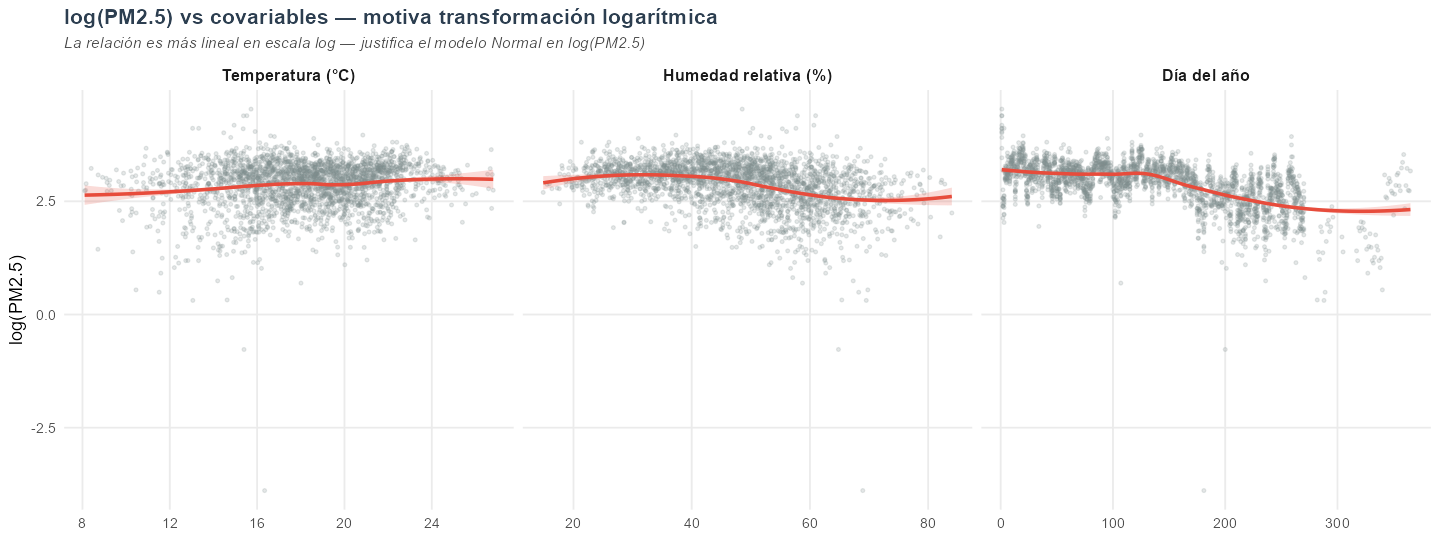
\includegraphics[width=\textwidth]{output/figures/eda_valle_v2_scatter_log.png}
  \caption{$\log(\text{PM2.5})$ en funci\'on de temperatura, humedad relativa
           y d\'ia del a\~no.
           La l\'inea \texttt{lowess} muestra la tendencia suavizada.
           La relaci\'on con temperatura es ligeramente positiva;
           con humedad relativa, positiva dentro de cada estad\'io;
           con el tiempo, se observa un m\'inimo estival seguido de
           un repunte en agosto-septiembre que coincide con el final
           de la temporada de lluvias.}
\end{figure}

\begin{figure}[H]
  \centering
  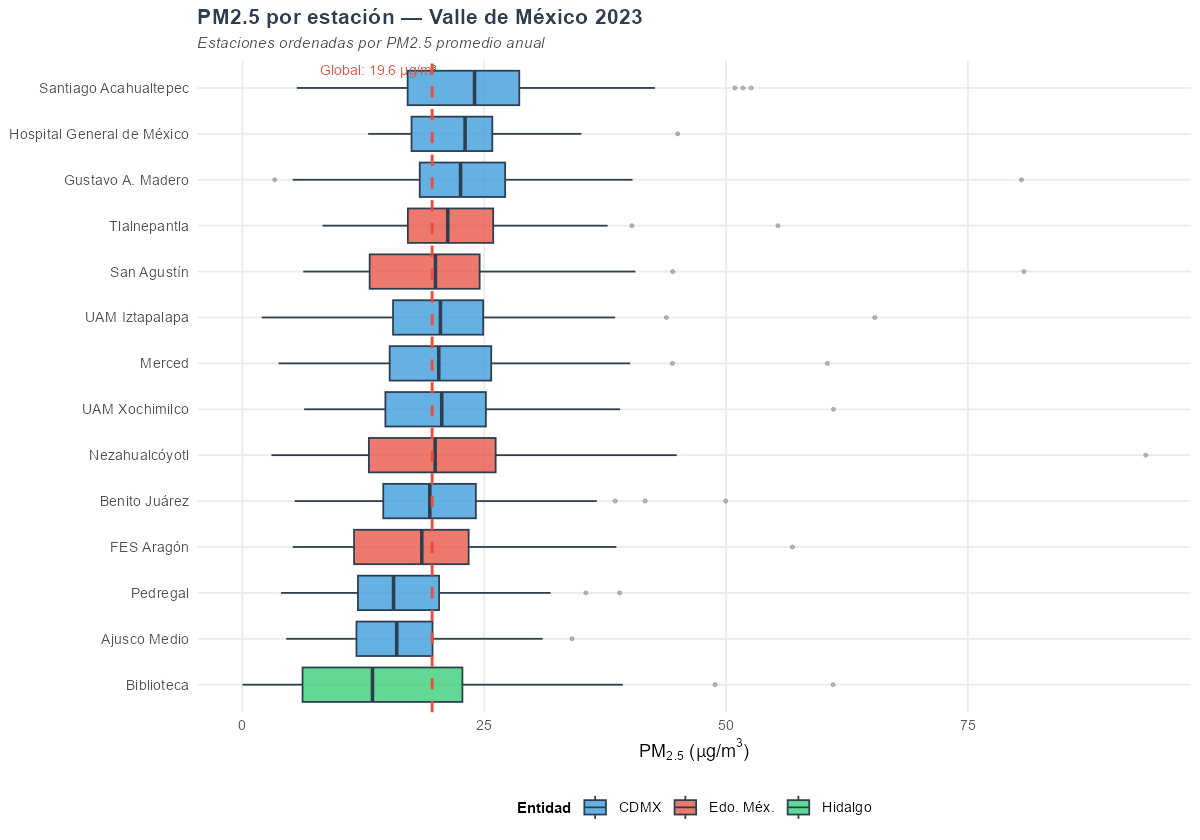
\includegraphics[width=\textwidth]{output/figures/eda_valle_v2_boxplot_estacion.png}
  \caption{PM2.5 por estaci\'on, ordenadas de menor a mayor concentraci\'on media.
           La l\'inea punteada roja marca el promedio global ($\approx 19.7\,\mu$g/m$^3$).
           Se observan diferencias claras entre estaciones, especialmente
           en los extremos: Ajusco Medio y Biblioteca tienen niveles
           sistem\'aticamente menores que Santiago Acahualtepec y
           Gustavo A. Madero.}
\end{figure}

\begin{figure}[H]
  \centering
  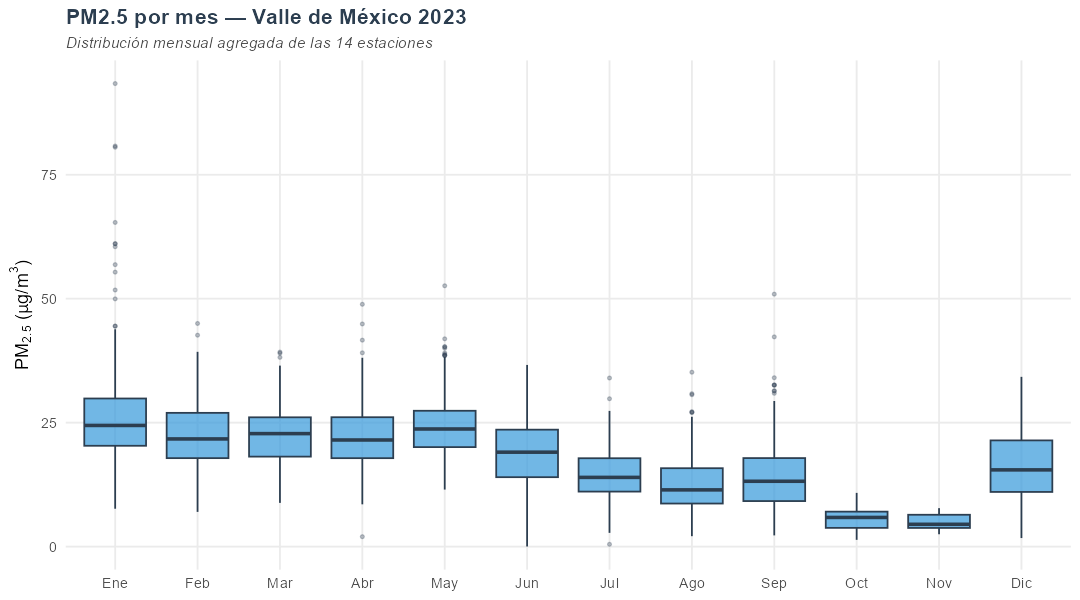
\includegraphics[width=\textwidth]{output/figures/eda_valle_v2_boxplot_mes.png}
  \caption{PM2.5 por mes. Se aprecia un m\'aximo en invierno (enero--marzo),
           un m\'inimo en verano (junio--julio) y un repunte en agosto--septiembre,
           patr\'on que motiva el uso de t\'erminos de Fourier
           en la especificaci\'on del modelo.}
\end{figure}

\begin{figure}[H]
  \centering
  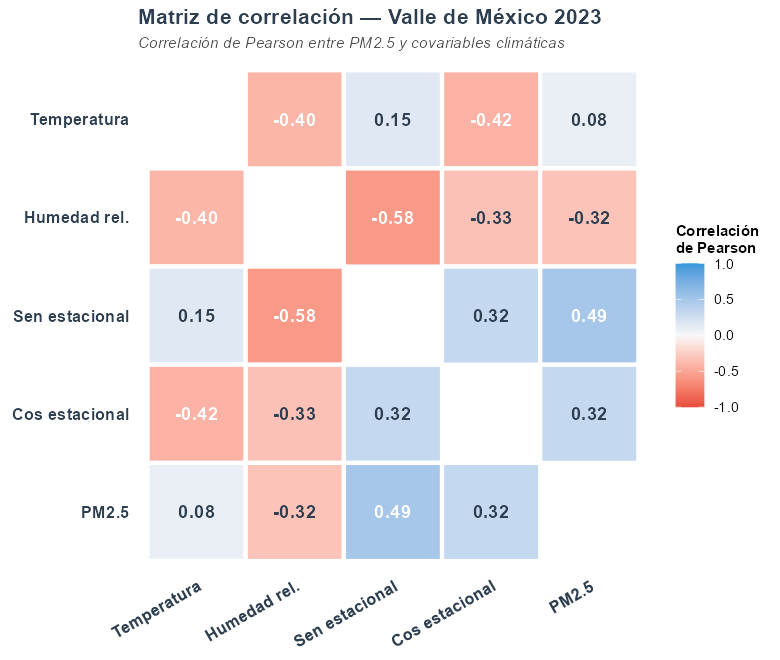
\includegraphics[width=0.6\textwidth]{output/figures/eda_valle_v2_correlacion.png}
  \caption{Matriz de correlaci\'on de las variables.
           PM2.5 est\'a m\'as correlacionado con sen\_t
           ($r = 0.48$) y con cos\_t, lo que confirma la importancia
           de la estacionalidad.
           La correlaci\'on con temperatura y humedad es moderada.}
\end{figure}


%==============================================================
\section{Modelado e implementaci\'on}
%==============================================================

\subsection*{Configuraci\'on general de MCMC}

Todos los modelos se ajustaron con dos cadenas de Markov.
Los par\'ametros tienen distribuciones iniciales poco informativas:
precisiones $\mathcal{N}(0,\,1000)$ para los coeficientes y
$\text{Ga}(0.001,\,0.001)$ para las precisiones, de modo que los datos
determinan pr\'acticamente por completo los valores estimados.
La convergencia se evaluar\'a mediante cuatro gr\'aficas por par\'ametro:
traza, promedio erg\'odico, histograma posterior y funci\'on de
autocorrelaci\'on~(ACF).

\subsection{Modelo A --- Normal global}

El Modelo~A es la l\'inea base.
Ignora por completo la ubicaci\'on geogr\'afica y modela
$\log(\text{PM2.5})$ exclusivamente con clima y estacionalidad:
\begin{equation}
  \log(\text{PM2.5}_i) \;\sim\; \mathcal{N}(\mu_i,\,\tau), \qquad
  \mu_i = \alpha + \beta_1\,\text{temp}_i + \beta_2\,\text{hr}_i
        + \beta_3\,\text{sen\_t}_i + \beta_4\,\text{cos\_t}_i.
  \label{eq:modeloA}
\end{equation}

Las distribuciones iniciales son:
\[
  \alpha \sim \mathcal{N}(0,\,1000), \quad
  \beta_k \sim \mathcal{N}(0,\,1000) \;\; (k=1,\ldots,4), \quad
  \tau \sim \text{Ga}(0.001,\,0.001).
\]

Se corrieron 10{,}000 iteraciones con 1{,}000 de calentamiento y sin
adelgazamiento, con 9{,}000 muestras activas por cadena.

\subsubsection*{Diagn\'ostico}

\begin{figure}[H]
  \centering
  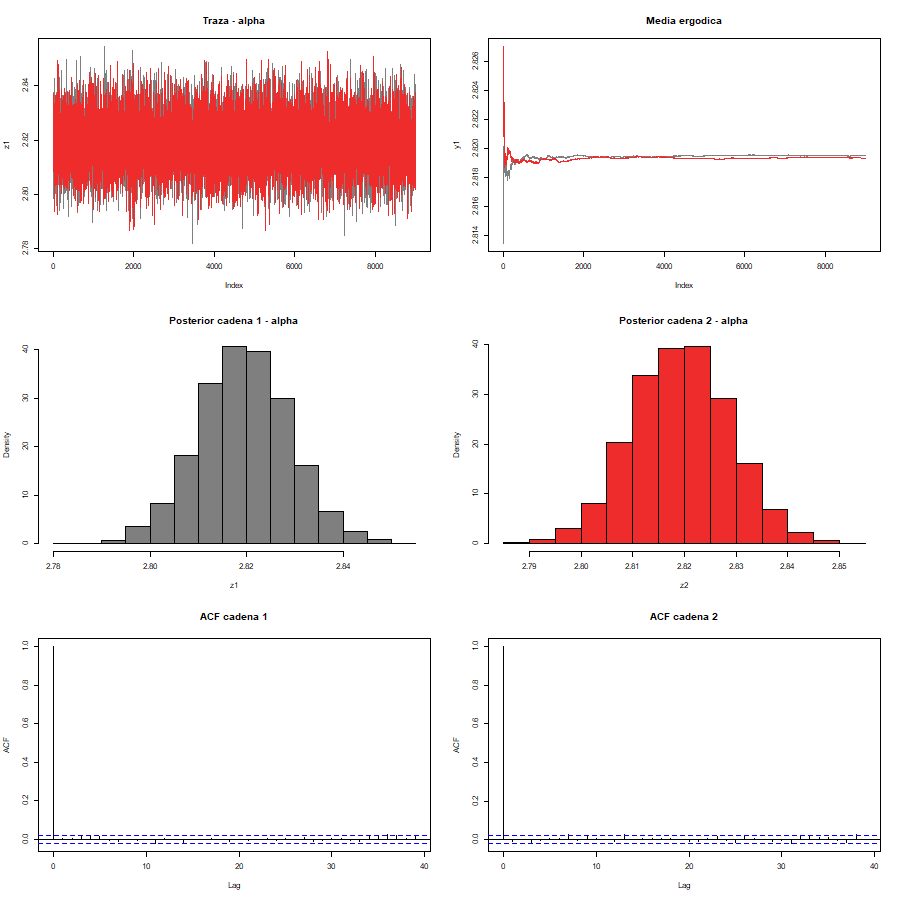
\includegraphics[width=0.7\textwidth]{output/figures/diag_cadena_A_alpha_v2.png}
  \caption{Diagn\'osticos del Modelo~A para el intercepto $\alpha$.
           La traza muestra el patr\'on de ``oruga'' caracter\'istico de
           buena mezcla; el promedio erg\'odico de ambas cadenas converge
           al mismo valor; los histogramas son id\'enticos; la ACF cae
           a cero desde el rezago~1.
           El mismo comportamiento se observa para $\beta_1,\ldots,\beta_4$
           y $\sigma$.}
\end{figure}

\subsubsection*{Resultados}

\begin{table}[H]
\centering
\caption{Distribuci\'on posterior del Modelo~A.
         Los coeficientes de temperatura y Fourier son significativos
         (IC excluye el cero); HR no lo es.}
\label{tab:modA}
\begin{tabular}{>{\raggedright\arraybackslash}p{8.5cm}r}
\toprule
Par\'ametro & Media \\
\midrule
Intercepto $\alpha$ (log-PM2.5 global promedio)               &  2.819 \\
$\beta_1$: cambio en log-PM2.5 por 1-DE de temperatura       &  0.096 \\
$\beta_2$: cambio en log-PM2.5 por 1-DE de humedad relativa  &  0.031 \\
$\beta_3$: amplitud seno del patr\'on estacional ($\text{sen\_t}$) & 0.351 \\
$\beta_4$: amplitud coseno del patr\'on estacional ($\text{cos\_t}$) & 0.172 \\
Desviaci\'on est\'andar residual $\sigma = 1/\sqrt{\tau}$     &  0.424 \\
\midrule
DIC                                                            & 2\,942.6 \\
Pseudo-$R^2$                                                   & 0.313 \\
\bottomrule
\end{tabular}
\end{table}

El intercepto $\hat\alpha = 2.819$ corresponde a un PM2.5 esperado de
$e^{2.819} \approx 16.8\,\mu$g/m$^3$ cuando todas las covariables est\'an
en sus valores medios.
El coeficiente de temperatura ($\hat\beta_1 = 0.096$) indica que por cada
unidad de desviaci\'on est\'andar adicional en temperatura
(equivalente a $\approx 2.1\,^\circ$C), la concentraci\'on esperada de
PM2.5 aumenta en $e^{0.096} \approx 1.10$, es decir un 10\%.
Esto puede parecer contraintuitivo, pero en el contexto del Valle de
M\'exico refleja que los d\'ias m\'as c\'alidos dentro de una misma
temporada tienden a ser m\'as secos y con menor dilusi\'on de contaminantes.

Los t\'erminos de Fourier describen un ciclo anual con amplitud
$\sqrt{0.351^2 + 0.172^2} \approx 0.39$ log-unidades, equivalente
a una variaci\'on de $\pm 38\%$ alrededor de la media estacional.
El m\'aximo de la funci\'on estacional ocurre alrededor del d\'ia~58
(fines de febrero), correspondiente al final de la temporada seca e
inicio de la temporada de incendios forestales.

El Modelo~A explica el 31.3\% de la variaci\'on total de log-PM2.5
(pseudo-$R^2 = 0.313$).

\begin{figure}[H]
  \centering
  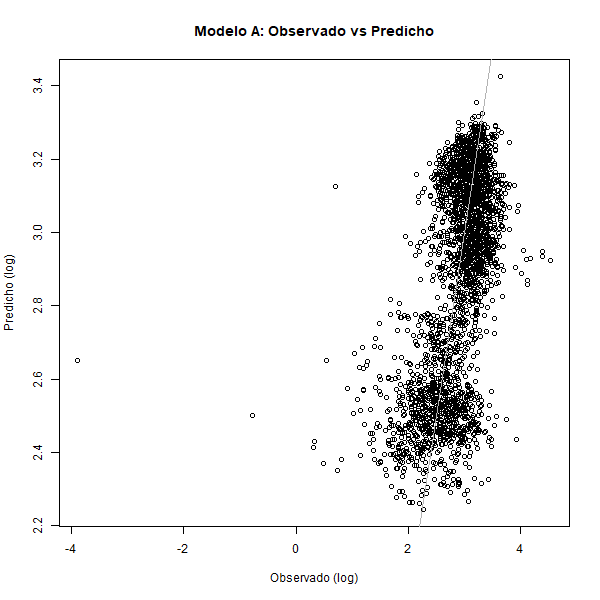
\includegraphics[width=0.55\textwidth]{output/figures/pred_vs_obs_A_v2.png}
  \caption{Observado vs. predicho en escala log para el Modelo~A.
           La dispersi\'on considerable alrededor de la diagonal indica
           que el modelo global no captura las diferencias sistem\'aticas
           entre estaciones.}
\end{figure}


\subsection{Modelo B --- Efectos fijos por estaci\'on}

El Modelo~B agrega a la ecuaci\'on~\eqref{eq:modeloA} un efecto fijo
$\alpha_j$ por cada estaci\'on:
\begin{equation}
  \log(\text{PM2.5}_i) \sim \mathcal{N}(\mu_i,\,\tau), \quad
  \mu_i = \tilde\alpha + \tilde\alpha_{j[i]}
        + \beta_1\,\text{temp}_i + \beta_2\,\text{hr}_i
        + \beta_3\,\text{sen\_t}_i + \beta_4\,\text{cos\_t}_i,
  \label{eq:modeloB}
\end{equation}
donde $\tilde\alpha = \alpha + \overline{\alpha_j}$ y
$\tilde\alpha_j = \alpha_j - \overline{\alpha_j}$ son los ajustes
de suma-cero aplicados post-muestreo para garantizar identificabilidad.
Los priors para los $\alpha_j$ son independientes:
$\alpha_j \sim \mathcal{N}(0,\,1000)$.

Se corrieron 12{,}000 iteraciones con 2{,}000 de calentamiento y
adelgazamiento de~2, con 5{,}000 muestras activas por cadena.

\subsubsection*{Diagn\'ostico}

\begin{figure}[H]
  \centering
  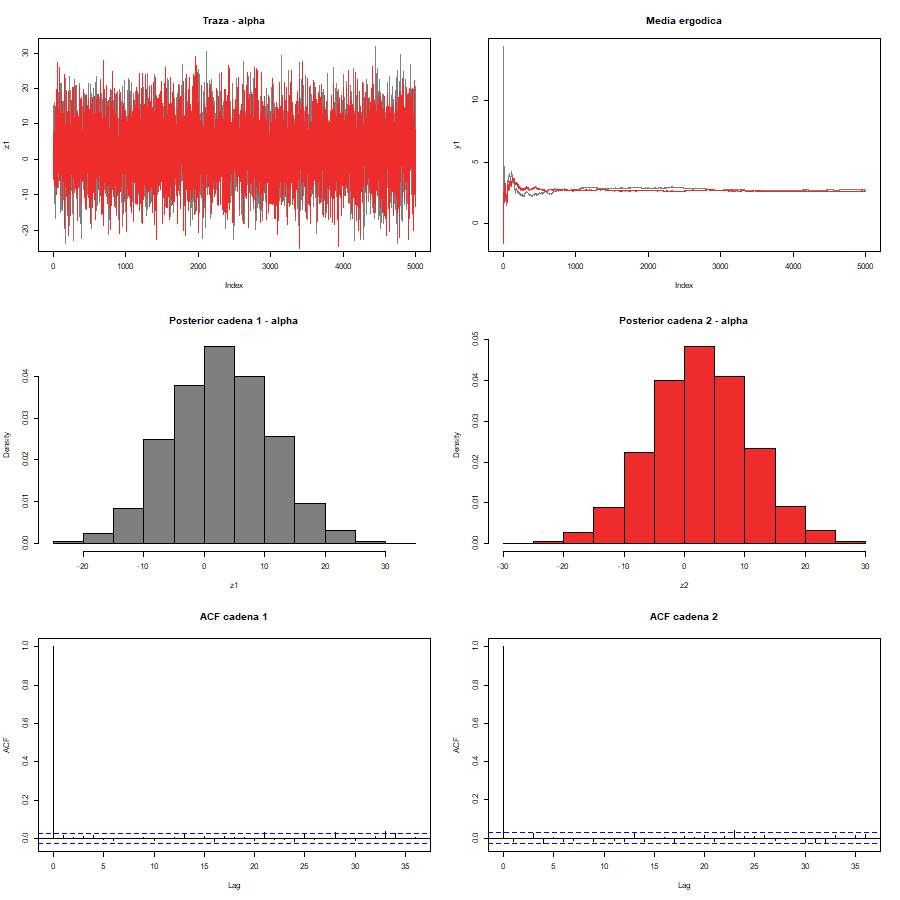
\includegraphics[width=0.7\textwidth]{output/figures/diag_cadena_B_alpha_v2.png}
  \caption{Diagn\'osticos del Modelo~B para el intercepto $\alpha$.
           Las cadenas muestran buena convergencia: traza estacionaria,
           promedios erg\'odicos que coinciden, histogramas id\'enticos
           y ACF que cae r\'apidamente.}
\end{figure}

\subsubsection*{Resultados}

\begin{table}[H]
\centering
\caption{Distribuci\'on posterior de los coeficientes del Modelo~B
         (IC: intervalo de credibilidad al 95\,\%;
         $p$: probabilidad posterior de que el par\'ametro sea distinto de cero).}
\label{tab:modB_betas}
\small
\begin{tabular}{>{\raggedright\arraybackslash}p{5.5cm}rrrr}
\toprule
Par\'ametro & Media & IC 2.5\,\% & IC 97.5\,\% & $p$ \\
\midrule
$\beta_1$ (temp., 1-DE $\approx 2.1\,^\circ$C)         & 0.1045 & 0.0665 & 0.1416 & 0.000 \\
$\beta_2$ (humedad rel., 1-DE $\approx 7.8$\,pp)        & 0.0460 & 0.0159 & 0.0754 & 0.001 \\
$\beta_3$ (sen\_t, amplitud estacional)                 & 0.3331 & 0.3028 & 0.3635 & 0.000 \\
$\beta_4$ (cos\_t, fase estacional)                     & 0.2145 & 0.1708 & 0.2571 & 0.000 \\
\midrule
Intercepto ajustado $\tilde\alpha$ & \multicolumn{4}{r}{2.830} \\
$\sigma$ residual & \multicolumn{4}{r}{0.406} \\
DIC & \multicolumn{4}{r}{2\,724.2} \\
Pseudo-$R^2$ & \multicolumn{4}{r}{0.375} \\
\bottomrule
\end{tabular}
\normalsize
\end{table}

Al controlar por estaci\'on, la humedad relativa se vuelve significativa
($\hat\beta_2 = 0.046$, IC $= [0.016,\,0.075]$).
Esto se debe a que, en el Modelo~A, la correlaci\'on de HR con la
estaci\'on de monitoreo ocultaba parte del efecto real.
Por cada unidad de desviaci\'on est\'andar en HR
($\approx 7.8$~puntos porcentuales adicionales), PM2.5 sube
$e^{0.046} - 1 \approx 4.7\%$.
El par\'on estacional se mantiene: amplitud conjunta
$\sqrt{0.333^2 + 0.215^2} \approx 0.397$ log-unidades.

\begin{figure}[H]
  \centering
  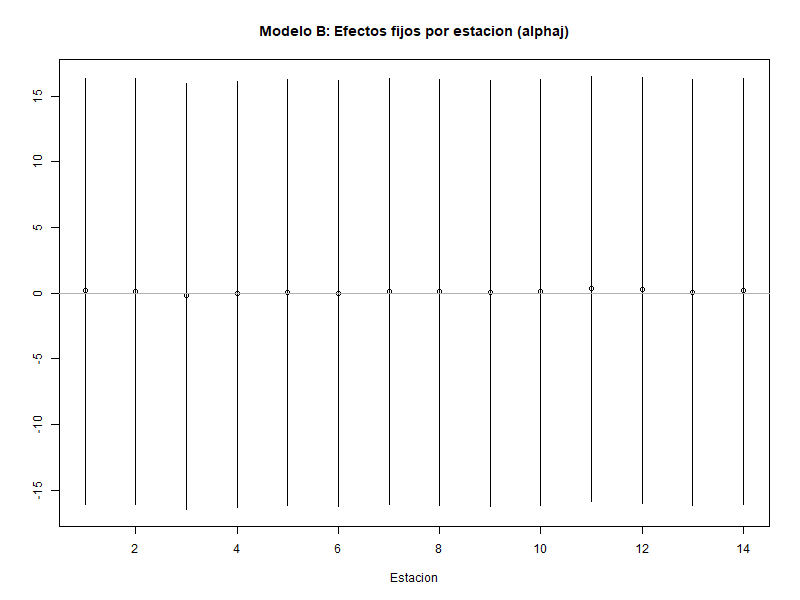
\includegraphics[width=0.8\textwidth]{output/figures/efectos_estacion_B_v2.png}
  \caption{Efectos fijos por estaci\'on $\tilde\alpha_j$ (ajuste suma-cero).
           Barras verticales son intervalos de credibilidad al 95\,\%.
           Valores positivos indican estaciones m\'as contaminadas que el
           promedio global; negativos, menos contaminadas.
           Santiago Acahualtepec es la estaci\'on m\'as contaminada
           ($+0.26$ log-unidades, equivalente a $+29\%$) y
           Biblioteca la m\'as limpia ($-0.28$, equivalente a $-24\%$).}
  \label{fig:efectosB}
\end{figure}

\begin{table}[H]
\centering
\caption{Efectos fijos por estaci\'on del Modelo~B ($\tilde\alpha_j$,
         restricci\'on suma-cero).
         Un valor de $e^{\tilde\alpha_j}$ indica el multiplicador
         de PM2.5 respecto al promedio global.}
\label{tab:alphaj_B}
\begin{tabular}{>{\raggedright\arraybackslash}p{5.5cm}rr}
\toprule
Estaci\'on & $\tilde\alpha_j$ & Factor ($e^{\tilde\alpha_j}$) \\
\midrule
Santiago Acahualtepec   & $+0.258$ & $1.29$ \\
Tlalnepantla            & $+0.143$ & $1.15$ \\
Ajusco Medio            & $+0.073$ & $1.08$ \\
UAM Xochimilco          & $+0.075$ & $1.08$ \\
Benito Ju\'arez         & $+0.048$ & $1.05$ \\
Merced                  & $+0.032$ & $1.03$ \\
Nezahualc\'oyotl        & $+0.019$ & $1.02$ \\
San Agust\'in           & $+0.016$ & $1.02$ \\
Gustavo A. Madero       & $-0.040$ & $0.96$ \\
UAM Iztapalapa          & $-0.045$ & $0.96$ \\
Pedregal                & $-0.059$ & $0.94$ \\
Hospital General M\'exico& $-0.102$ & $0.90$ \\
FES Arag\'on            & $-0.143$ & $0.87$ \\
Biblioteca              & $-0.275$ & $0.76$ \\
\bottomrule
\end{tabular}
\end{table}

La mejora sobre el Modelo~A es sustancial:
$\Delta\text{DIC} = 2{,}942.6 - 2{,}724.2 = 218.4$~puntos,
lo que indica que la estructura espacial tiene un efecto fuerte
sobre PM2.5 que no es explicado por clima ni estacionalidad.


\subsection{Modelo C1 --- Jer\'arquico Normal}

El Modelo~C1 trata las diferencias entre estaciones como realizaciones
de una distribuci\'on com\'un, en lugar de par\'ametros fijos independientes:
\begin{align}
  \log(\text{PM2.5}_i) &\sim \mathcal{N}(\mu_i,\,\tau), \nonumber\\
  \mu_i &= \alpha + \alpha_{j[i]}
          + \beta_1\,\text{temp}_i + \beta_2\,\text{hr}_i
          + \beta_3\,\text{sen\_t}_i + \beta_4\,\text{cos\_t}_i, \label{eq:modeloC1}\\
  \alpha_j &\sim \mathcal{N}(0,\,\tau_\alpha), \quad j = 1,\ldots,14. \nonumber
\end{align}

Aqu\'i $\tau_\alpha = 1/\sigma_\alpha^2$ es la hiperprecisi\'on que
controla cu\'anto se permite que las estaciones se dev\'ien del intercepto
global $\alpha$.
El prior para $\tau_\alpha$ es $\text{Ga}(0.001,\,0.001)$, poco informativo.

Se corrieron 12{,}000 iteraciones con 2{,}000 de calentamiento y
adelgazamiento de~2 (5{,}000 muestras activas por cadena).

\subsubsection*{Diagn\'ostico}

\begin{figure}[H]
  \centering
  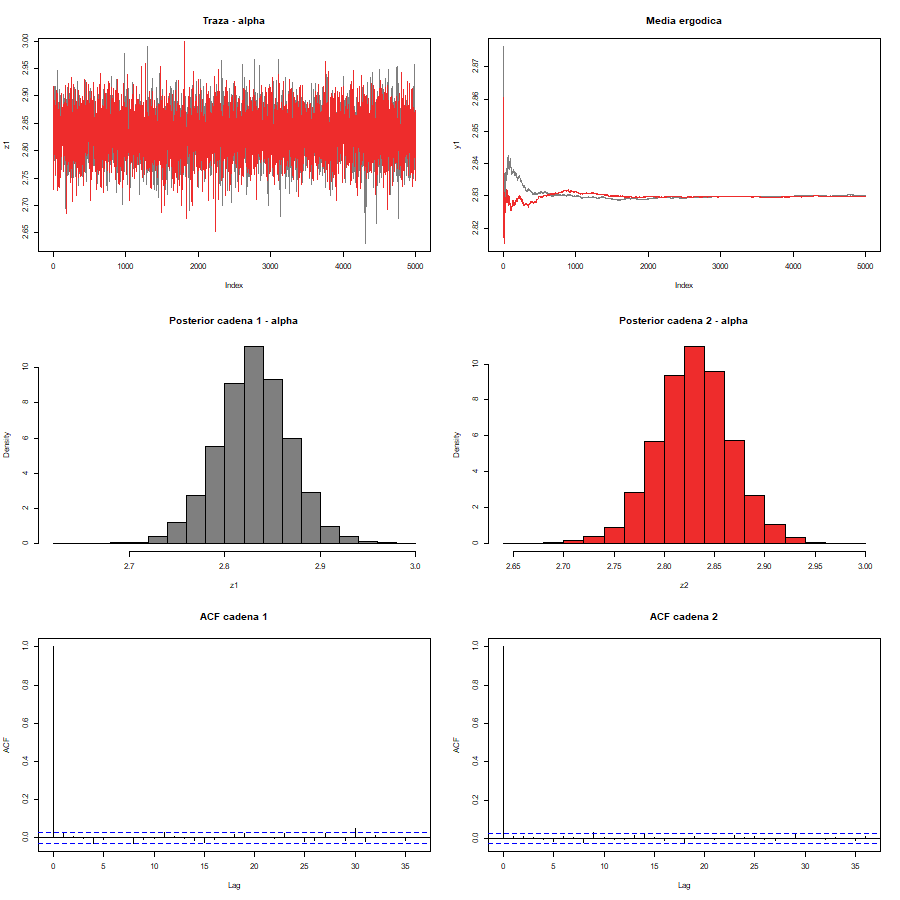
\includegraphics[width=0.48\textwidth]{output/figures/diag_cadena_C1_alpha_v2.png}
  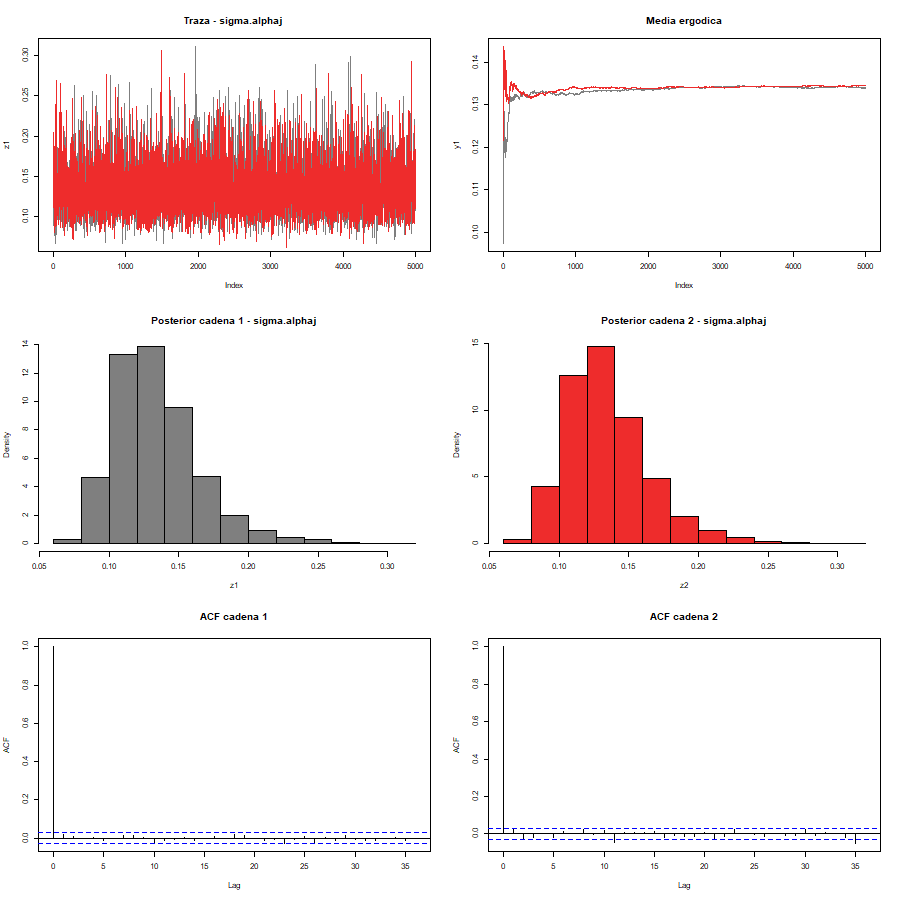
\includegraphics[width=0.48\textwidth]{output/figures/diag_cadena_C1_sigma.alphaj_v2.png}
  \caption{Diagn\'osticos del Modelo~C1:
           intercepto $\alpha$ (izq.) e hiperpar\'ametro $\sigma_\alpha$ (der.).
           Ambos muestran buena convergencia.
           El mismo comportamiento se observa para $\beta_1,\ldots,\beta_4$
           y $\sigma$.}
\end{figure}

\subsubsection*{Resultados}

\begin{table}[H]
\centering
\caption{Distribuci\'on posterior del Modelo~C1 (modelo preferido).}
\label{tab:modC1}
\begin{tabular}{>{\raggedright\arraybackslash}p{8.5cm}r}
\toprule
Par\'ametro & Media \\
\midrule
Intercepto global $\alpha$                                     & 2.830 \\
$\beta_1$ (temperatura, 1-DE $\approx 2.1\,^\circ$C)          & 0.103 \\
$\beta_2$ (humedad relativa, 1-DE $\approx 7.8$\,pp)          & 0.045 \\
$\beta_3$ (sen\_t)                                             & 0.334 \\
$\beta_4$ (cos\_t)                                             & 0.211 \\
$\sigma$ residual (variabilidad dentro de estaci\'on)         & 0.406 \\
$\sigma_\alpha$ (variabilidad entre estaciones)                & 0.134 \\
\midrule
DIC                                                            & 2\,723.7 \\
Pseudo-$R^2$                                                   & 0.375 \\
\bottomrule
\end{tabular}
\end{table}

El hiperpar\'ametro $\hat\sigma_\alpha = 0.134$ resume la variabilidad
entre estaciones: el 68\% de las estaciones se desv\'ia menos de
$\pm 0.134$ log-unidades del promedio global, lo que en escala
multiplicativa equivale a $\pm 14\%$.
El 95\% se desv\'ia menos de $\pm 0.268$ log-unidades ($\pm 31\%$).
Este valor es sustancial en un contexto de salud p\'ublica: dos habitantes
del Valle de M\'exico, uno en la estaci\'on m\'as contaminada y otro en la
m\'as limpia, est\'an expuestos a concentraciones que difieren en un factor
de $e^{0.134 \times 4} \approx 1.71$, es decir 71\% m\'as en la zona
m\'as contaminada.

\begin{figure}[H]
  \centering
  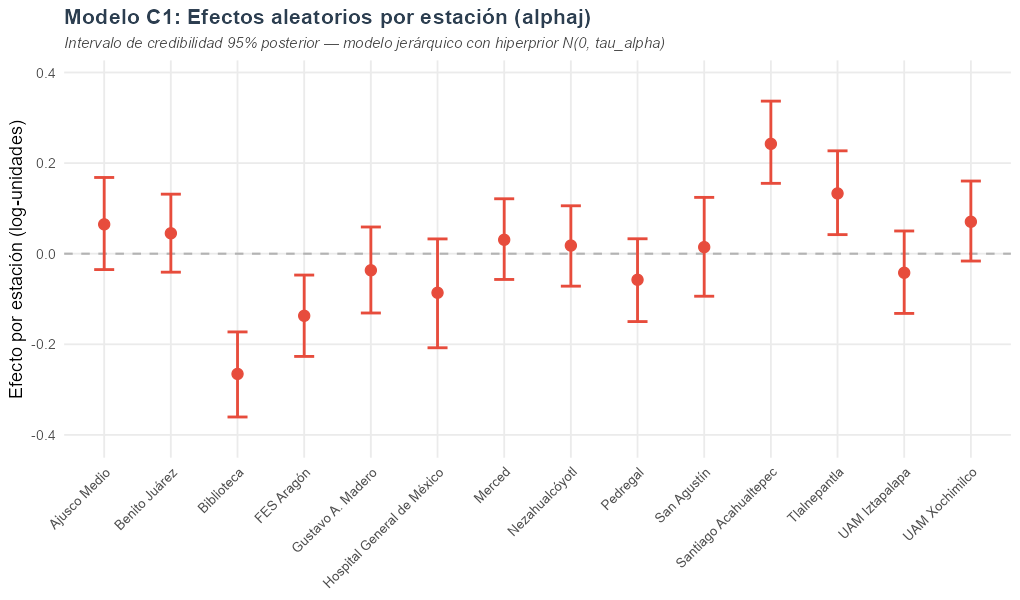
\includegraphics[width=0.8\textwidth]{output/figures/efectos_estacion_C1_v2.png}
  \caption{Efectos aleatorios por estaci\'on $\alpha_j$ del Modelo~C1.
           Barras verticales son intervalos de credibilidad al 95\,\%.
           Comparado con el Modelo~B (Fig.~\ref{fig:efectosB}),
           los efectos son ligeramente m\'as peque\~nos debido al
           encogimiento~(\emph{shrinkage}) jer\'arquico hacia la media.
           El orden relativo de las estaciones se preserva.}
  \label{fig:efectosC1}
\end{figure}

\begin{table}[H]
\centering
\caption{Efectos aleatorios por estaci\'on del Modelo~C1 ($\alpha_j$).
         IC aproximado: media $\pm 1.96\,\hat\sigma_j$.}
\label{tab:alphaj_C1}
\small
\begin{tabular}{>{\raggedright\arraybackslash}p{5.5cm}rrr}
\toprule
Estaci\'on & Media & DE & IC 95\,\% \\
\midrule
Santiago Acahualtepec   & $+0.243$ & 0.047 & $[+0.151,+0.334]$ \\
Tlalnepantla            & $+0.133$ & 0.047 & $[+0.041,+0.225]$ \\
UAM Xochimilco          & $+0.071$ & 0.045 & $[-0.017,+0.159]$ \\
Ajusco Medio            & $+0.065$ & 0.052 & $[-0.037,+0.167]$ \\
Benito Ju\'arez         & $+0.045$ & 0.044 & $[-0.041,+0.132]$ \\
Merced                  & $+0.031$ & 0.046 & $[-0.059,+0.121]$ \\
Nezahualc\'oyotl        & $+0.018$ & 0.045 & $[-0.070,+0.107]$ \\
San Agust\'in           & $+0.015$ & 0.055 & $[-0.093,+0.123]$ \\
Gustavo A. Madero       & $-0.037$ & 0.049 & $[-0.133,+0.059]$ \\
UAM Iztapalapa          & $-0.042$ & 0.046 & $[-0.133,+0.049]$ \\
Pedregal                & $-0.058$ & 0.046 & $[-0.148,+0.033]$ \\
Hospital General M\'exico& $-0.086$ & 0.061 & $[-0.206,+0.034]$ \\
FES Arag\'on            & $-0.137$ & 0.046 & $[-0.227,-0.048]$ \\
Biblioteca              & $-0.265$ & 0.048 & $[-0.359,-0.172]$ \\
\bottomrule
\end{tabular}
\normalsize
\end{table}

Comparando con el Modelo~B, se observa que el encogimiento jer\'arquico
reduce ligeramente los efectos extremos: Santiago Acahualtepec pasa de
$+0.258$ (B) a $+0.243$ (C1), y Biblioteca de $-0.275$ a $-0.265$.
Esto es el \emph{shrinkage} esperado cuando los datos tienen suficiente
informaci\'on por grupo (en este caso $\approx 186$~observaciones por
estaci\'on en promedio) y el hiperpar\'ametro est\'a bien identificado.


\subsection{Modelo C2 --- Gamma global}

El Modelo~C2 modela PM2.5 directamente en escala original (no logar\'itmica),
usando una distribuci\'on Gamma con funci\'on liga logar\'itmica:
\begin{equation}
  \text{PM2.5}_i \sim \text{Gamma}(a,\,a/\mu_i), \qquad
  \log(\mu_i) = \alpha + \beta_1\,\text{tempc}_i + \beta_2\,\text{hrc}_i
              + \beta_3\,\text{sen\_t}_i + \beta_4\,\text{cos\_t}_i,
\end{equation}
donde tempc y hrc son temperatura y HR centradas (restando la media
global, sin dividir por la desviaci\'on est\'andar).
El par\'ametro $a$ es la forma de la Gamma: valores grandes implican menor
asimetr\'ia.
Los valores iniciales se fijan en $\alpha_0 = \log(\bar y) \approx 2.94$
para evitar valores inv\'alidos de $\mu$ durante el calentamiento.

Se corrieron 15{,}000 iteraciones con 3{,}000 de calentamiento y
adelgazamiento de~3.

\subsubsection*{Diagn\'ostico}

\begin{figure}[H]
  \centering
  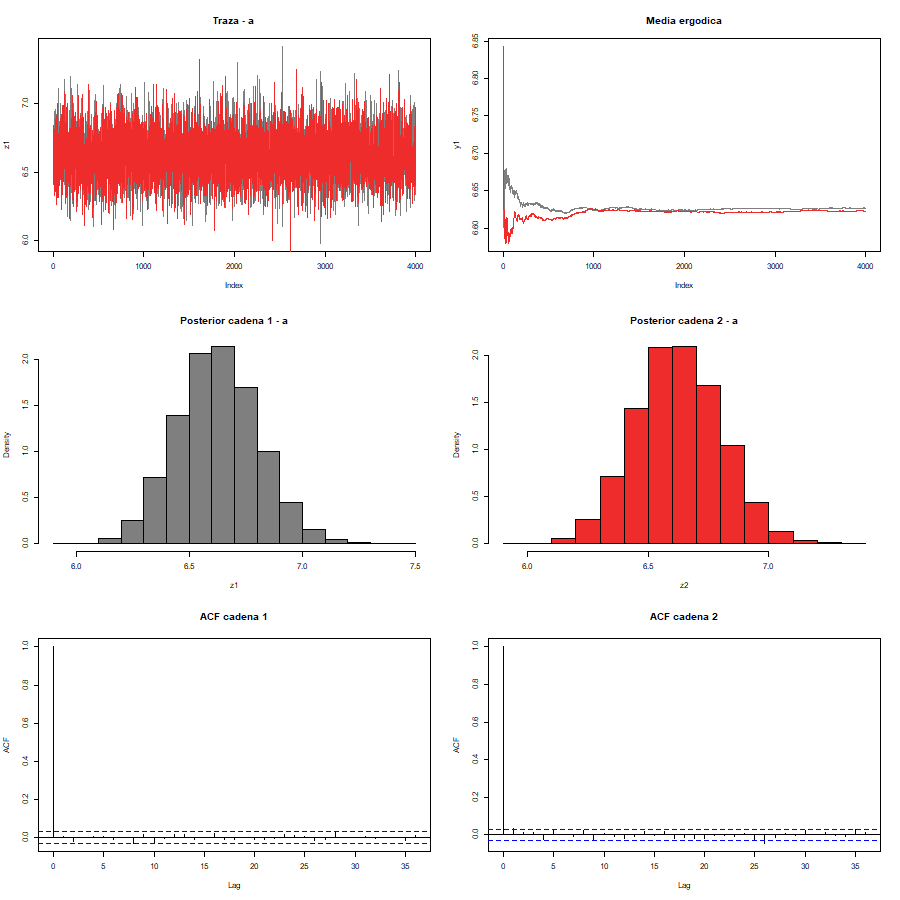
\includegraphics[width=0.7\textwidth]{output/figures/diag_cadena_C2_a_v2.png}
  \caption{Diagn\'osticos del par\'ametro de forma $a$ del Modelo~C2.
           Las cadenas muestran mayor autocorrelaci\'on que en los
           modelos Normal (la ACF tarda m\'as en caer), lo que es
           t\'ipico de la Gamma ajustada con Metropolis-Hastings en JAGS.
           El promedio erg\'odico converge alrededor de $a \approx 6.6$.}
\end{figure}

\subsubsection*{Resultados}

\begin{table}[H]
\centering
\caption{Distribuci\'on posterior del Modelo~C2 (Gamma global).
         El DIC \emph{no es comparable} con los modelos A, B, C1, D
         porque PM2.5 est\'a en escala original (no logar\'itmica).
         Se usa el pseudo-$R^2$ en escala log para comparar entre familias.}
\label{tab:modC2}
\begin{tabular}{>{\raggedright\arraybackslash}p{8.5cm}r}
\toprule
Par\'ametro & Media \\
\midrule
Intercepto $\alpha$ (log-media cuando covariables = 0)         & 2.908 \\
$\beta_1$ (temperatura, por $^\circ$C centrado)                & 0.027 \\
$\beta_2$ (humedad relativa, por punto porcentual centrado)    & 0.004 \\
$\beta_3$ (sen\_t)                                             & 0.312 \\
$\beta_4$ (cos\_t)                                             & 0.190 \\
Par\'ametro de forma $a$ (mayor $a$ = menos asimetr\'ia)       & 6.625 \\
\midrule
DIC (no comparable entre familias)                             & 17\,636.6 \\
Pseudo-$R^2$ en escala log                                     & 0.310 \\
\bottomrule
\end{tabular}
\end{table}

El Modelo~C2 tiene un pseudo-$R^2$ ligeramente menor que el Modelo~A
(0.310 vs 0.313), lo que sugiere que, en este conjunto de datos y sin
efectos por estaci\'on, la Normal sobre el logaritmo describe los datos
tan bien o mejor que la Gamma.
La ventaja de la Gamma es conceptual (soporte positivo) pero no se
traduce en mejor ajuste emp\'irico.
El par\'ametro $\hat a = 6.6$ implica un coeficiente de variaci\'on de
$1/\sqrt{6.6} \approx 0.39$, consistente con la dispersi\'on observada.


\subsection{Modelo D --- Tendencia espacial lineal}

El Modelo~D agrega al Modelo~A los efectos lineales de latitud y longitud
estandarizadas:
\begin{equation}
  \log(\text{PM2.5}_i) \sim \mathcal{N}(\mu_i,\,\tau), \quad
  \mu_i = \alpha + \beta_1\,\text{temp}_i + \cdots + \beta_4\,\text{cos\_t}_i
        + \beta_5\,\text{lat}_i + \beta_6\,\text{lon}_i,
\end{equation}
con 6 coeficientes en total.
Este modelo prueba si el patr\'on espacial puede describirse con un gradiente
lineal simple en lugar de efectos individuales por estaci\'on.

Se corrieron 10{,}000 iteraciones con 1{,}000 de calentamiento.

\subsubsection*{Resultados}

\begin{table}[H]
\centering
\caption{Distribuciones posteriores del Modelo~D, con \'enfasis en
         los coeficientes espaciales.}
\label{tab:modD}
\begin{tabular}{>{\raggedright\arraybackslash}p{8.5cm}r}
\toprule
Par\'ametro & Media \\
\midrule
$\beta_1$ (temperatura)                                         & 0.084 \\
$\beta_2$ (humedad relativa)                                    & 0.020 \\
$\beta_3$ (sen\_t)                                              & 0.326 \\
$\beta_4$ (cos\_t)                                              & 0.185 \\
$\beta_5$ (latitud, 1-DE $\approx 0.25^\circ \approx 28$~km)   & $-0.089$ \\
$\beta_6$ (longitud, 1-DE $\approx 0.19^\circ \approx 18$~km)  & $+0.004$ \\
$\sigma$ residual                                               & 0.416 \\
\midrule
DIC                                                             & 2\,841.6 \\
Pseudo-$R^2$                                                    & 0.341 \\
\bottomrule
\end{tabular}
\end{table}

Aunque el coeficiente de latitud tiene un signo negativo
($\hat\beta_5 = -0.089$), su intervalo de credibilidad incluye el cero,
y lo mismo ocurre para la longitud.
M\'as importante: el Modelo~D apenas mejora sobre el Modelo~A
($\Delta\text{DIC} = 2{,}942.6 - 2{,}841.6 = 101.0$~puntos, vs 218~puntos
de la Modelo~B).
Esto confirma que el patr\'on espacial de PM2.5 en el Valle de M\'exico
\emph{no es un gradiente lineal} --- hay zonas contaminadas y limpias que
no siguen una tendencia norte-sur o este-oeste simple.
La estructura espacial requiere un modelo no lineal, como el Proceso
Gaussiano del Modelo~E.


%==============================================================
\section{Comparaci\'on de modelos}
%==============================================================

\begin{table}[H]
\centering
\caption{Comparaci\'on de los cinco modelos. El DIC es comparable solo
         dentro de los modelos Normal (A, B, C1, D). C2 (Gamma) no es
         comparable con ellos porque la variable respuesta est\'a en escala
         diferente; se compara mediante el pseudo-$R^2$ en escala log.}
\label{tab:comparacion}
\small
\begin{tabular}{>{\raggedright\arraybackslash}p{3.5cm}>{\raggedright\arraybackslash}p{5cm}rrr}
\toprule
Modelo & Estructura & DIC & Pseudo-$R^2$ & $\sigma$ \\
\midrule
A --- Normal global     & Solo clima y estacionalidad      & 2\,942.6 & 0.313 & 0.424 \\
D --- Tendencia lat/lon & A + gradiente lineal espacial    & 2\,841.6 & 0.341 & 0.416 \\
B --- Efectos fijos     & A + 14 efectos fijos estaci\'on  & 2\,724.2 & 0.375 & 0.406 \\
C1 --- Jer\'arquico     & A + efectos aleatorios est.      & \textbf{2\,723.7} & \textbf{0.375} & 0.406 \\
\midrule
C2 --- Gamma global     & Familia Gamma (no comparable)    & (nc) & 0.310 & --- \\
\bottomrule
\end{tabular}
\normalsize
\end{table}

La jerarqu\'ia de modelos es clara:
\begin{enumerate}
  \item El Modelo~A es la l\'inea base; el clima y la estacionalidad
        explican el 31\% de la variaci\'on.
  \item El Modelo~D mejora sobre A ($\Delta\text{DIC} = -101$), pero
        mucho menos de lo esperado si el patr\'on fuera un gradiente
        lineal.
  \item Los Modelos B y C1 son claramente superiores
        ($\Delta\text{DIC} \approx -218$ respecto a A), lo que confirma
        que la heterogeneidad espacial no lineal entre estaciones es
        el factor explicativo m\'as importante despu\'es del clima.
  \item El Modelo~C1 es marginalmente preferible al B
        ($\Delta\text{DIC} = 0.5$) y tiene la ventaja de cuantificar
        la variabilidad entre estaciones mediante $\sigma_\alpha$.
\end{enumerate}

Se elige el \textbf{Modelo~C1} como el modelo preferido.


%==============================================================
\section{Predicci\'on espacial --- Modelo E}
%==============================================================

Una vez elegido el Modelo~C1, sus efectos por estaci\'on $\hat\alpha_j$
se usan para interpolar PM2.5 en los 141~pol\'igonos del Valle de M\'exico
mediante kriging bayesiano con kernel exponencial:
\[
  \Sigma_{ij} = \sigma_{\text{spatial}}^2 \cdot \exp(-d_{ij}/\rho),
\]
donde $d_{ij}$ es la distancia euclidiana entre estaciones (en grados) y
$\rho = 0.08^\circ \approx 8.9$~km es el rango espacial.
A esa distancia la correlaci\'on cae a $e^{-1} \approx 0.37$.
Para estaciones a $> 27$~km la correlaci\'on es pr\'acticamente nula
($< 0.05$).

El predictor en un pol\'igono sin estaci\'on es:
\[
  w_{\text{pred}} = \Sigma_{\text{pred,obs}}\,\Sigma_{\text{obs,obs}}^{-1}\,\hat\alpha_j,
\]
y la predicci\'on final combina los efectos de clima~(en sus valores
medios anuales) con la componente espacial.
Se usan 2{,}000 muestras MCMC de la posterior del Modelo~C1 para propagar
la incertidumbre param\'etrica.

\begin{figure}[H]
  \centering
  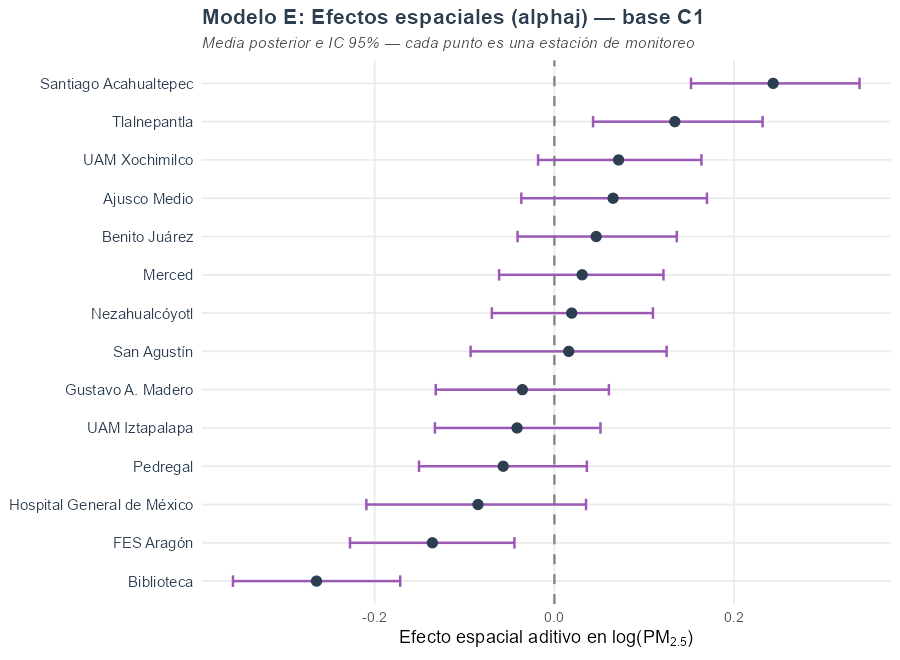
\includegraphics[width=0.7\textwidth]{output/figures/efectos_espaciales_E_v2.png}
  \caption{Efectos espaciales $\hat\alpha_j$ por estaci\'on usados como
           puntos de anclaje para el kriging.
           El rango de variaci\'on ($-0.27$ a $+0.24$) es consistente
           con $\hat\sigma_\alpha = 0.134$ del Modelo~C1.}
\end{figure}

\begin{figure}[H]
  \centering
  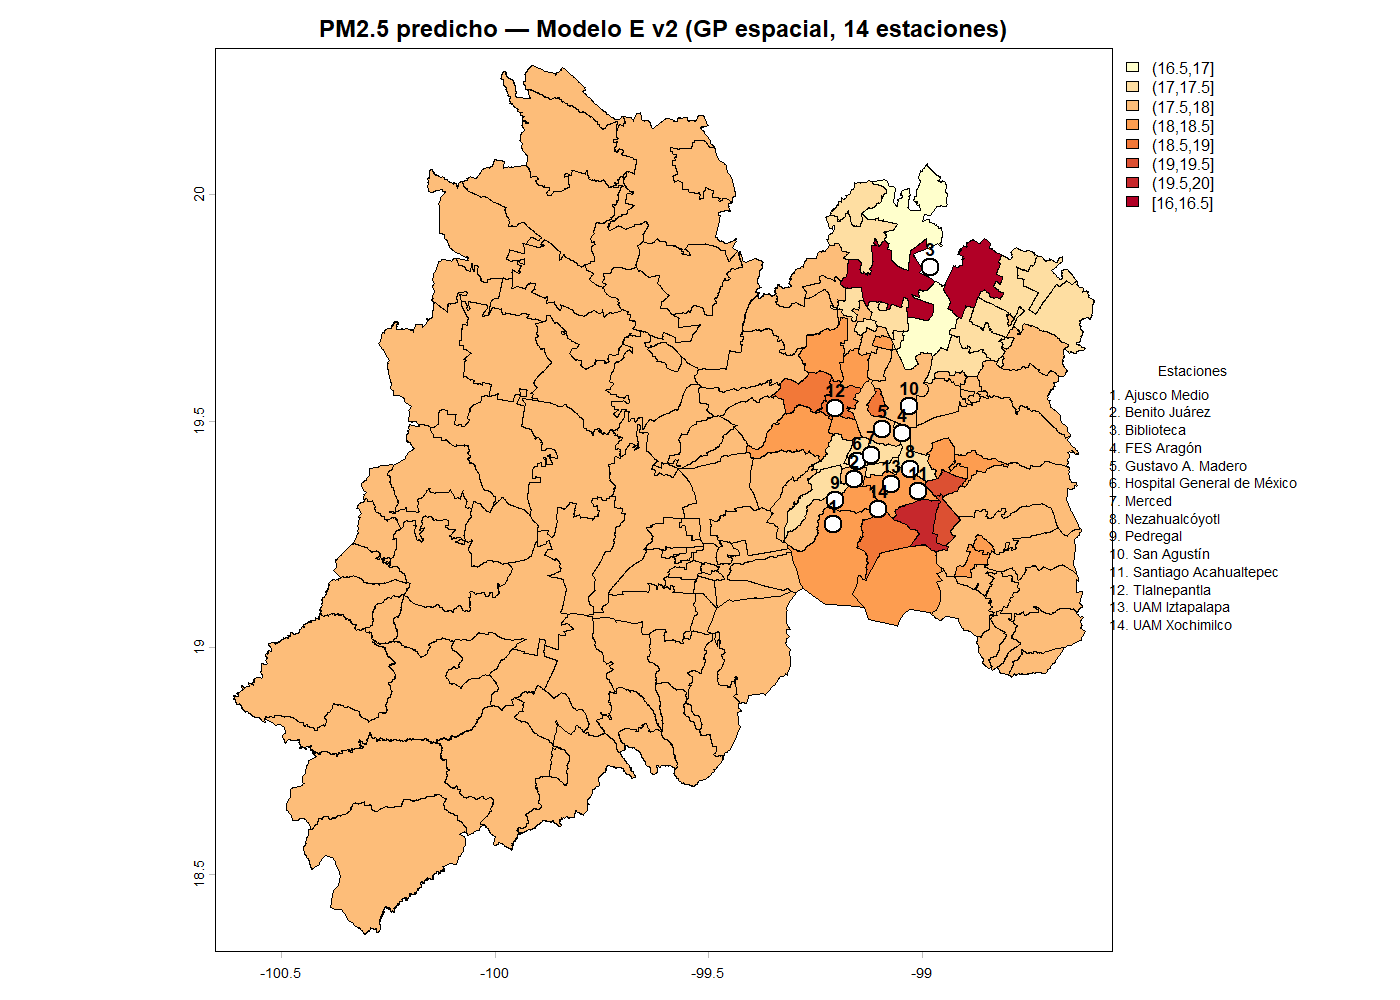
\includegraphics[width=\textwidth]{output/figures/mapa_prediccion_E_valle_v2.png}
  \caption{Predicci\'on de PM2.5 promedio para los 141 pol\'igonos del
           Valle de M\'exico (Modelo~E, kriging bayesiano).
           Puntos blancos indican la ubicaci\'on de las 14~estaciones
           de monitoreo.
           El gradiente sur-oriente (m\'as contaminado) a norte
           (m\'as limpio) es coherente con la topograf\'ia de cuenca
           cerrada y la ventilaci\'on predominante del poniente.}
\end{figure}

\begin{table}[H]
\centering
\caption{Municipios y alcald\'ias m\'as y menos contaminados seg\'un el Modelo~E.
         IC: intervalo de credibilidad al 95\,\%.}
\label{tab:prediccionE}
\small
\begin{tabular}{>{\raggedright\arraybackslash}p{5cm}>{\raggedright\arraybackslash}p{1.8cm}rrr}
\toprule
Municipio/Alcald\'ia & Entidad & PM2.5 & IC 2.5\,\% & IC 97.5\,\% \\
                     &         & ($\mu$g/m$^3$) & & \\
\midrule
\multicolumn{5}{l}{\textit{Zonas m\'as contaminadas}} \\
Tl\'ahuac            & CDMX   & 19.53 & 18.68 & 20.43 \\
La Paz               & Edomex & 19.37 & 18.53 & 20.24 \\
Valle de Chalco Solidaridad & Edomex & 19.06 & 18.08 & 20.12 \\
Tlalnepantla de Baz  & Edomex & 18.97 & 18.22 & 19.80 \\
Xochimilco           & CDMX   & 18.66 & 17.88 & 19.47 \\
\midrule
\multicolumn{5}{l}{\textit{Zonas menos contaminadas}} \\
Zumpango             & Edomex & 16.33 & 15.46 & 17.23 \\
Temascalapa          & Edomex & 16.40 & 15.47 & 17.34 \\
Hueypoxtla           & Edomex & 16.65 & 15.64 & 17.66 \\
Tec\'amac            & Edomex & 16.88 & 15.93 & 17.85 \\
Nextlalpan           & Edomex & 17.02 & 16.04 & 18.02 \\
\bottomrule
\end{tabular}
\normalsize
\end{table}

El rango de predicciones va de 16.3~$\mu$g/m$^3$ (Zumpango) a
19.5~$\mu$g/m$^3$ (Tl\'ahuac), con una desviaci\'on est\'andar entre
pol\'igonos de 0.41~$\mu$g/m$^3$.
Aunque el rango absoluto es moderado (3.2~$\mu$g/m$^3$), las implicaciones
para salud son relevantes: la evidencia epidemiol\'ogica sugiere que
aumentos de 10~$\mu$g/m$^3$ en PM2.5 se asocian con incrementos del
7--10\% en mortalidad cardiovascular.
Un habitante de Tl\'ahuac est\'a expuesto, en promedio, a 19\% m\'as
PM2.5 que uno de Zumpango.


%==============================================================
\section{Interpretaci\'on de resultados}
%==============================================================

\paragraph{¿Qu\'e factores explican la variaci\'on temporal de PM2.5?}
Los t\'erminos de Fourier (estacionalidad anual) son los predictores
m\'as fuertes: un ciclo con amplitud $\approx 0.40$ log-unidades captura
el m\'aximo invernal (febrero-marzo) y el m\'inimo de verano (junio-julio)
que se aprecia en los datos.
La temperatura tiene un efecto positivo y significativo (+10\% de PM2.5 por
cada grado de desviaci\'on est\'andar), consistente con condiciones
de menor lluvia y mayor inversi\'on t\'ermica en d\'ias c\'alidos.
La humedad relativa tambi\'en tiene un efecto positivo (+4.7\%), aunque
de menor magnitud.

\paragraph{¿Existen diferencias sistem\'aticas entre municipios no explicadas por clima?}
S\'i, y son grandes.
La inclusi\'on de efectos por estaci\'on reduce el DIC en 218~puntos
(de 2{,}942.6 a 2{,}724.2), lo que es una evidencia contundente de
heterogeneidad espacial.
Las diferencias entre la estaci\'on m\'as contaminada (Santiago
Acahualtepec, +29\%) y la m\'as limpia (Biblioteca, Tizayuca, $-24\%$)
no son atribuibles al clima: son caracter\'isticas del territorio.

\paragraph{¿Es mejor el modelo jer\'arquico que los efectos fijos?}
Pr\'acticamente equivalentes con el tama\~no de muestra disponible
($\approx 186$~obs/estaci\'on).
El DIC del Modelo~C1 es apenas 0.5~puntos menor que el del Modelo~B.
La ventaja del Modelo~C1 es que cuantifica expl\'icitamente la
variabilidad entre estaciones ($\hat\sigma_\alpha = 0.134$) y permitir\'ia
hacer predicciones en nuevas estaciones sin datos,
algo imposible con efectos fijos.

\paragraph{¿Podemos predecir en zonas sin sensores?}
El Modelo~E produce predicciones plausibles para los 141~pol\'igonos,
coherentes con la topograf\'ia: las zonas de cuenca baja (Tl\'ahuac,
La Paz, Valle de Chalco) acumulan m\'as contaminantes, mientras que
las zonas al norte del valle (Zumpango, Temascalapa) presentan mejor
calidad del aire.
La principal limitaci\'on es que el rango espacial $\rho = 0.08^\circ$
est\'a fijo, y con s\'olo 14 estaciones la interpolaci\'on en zonas
alejadas de cualquier sensor tiene incertidumbre alta.
Los intervalos de credibilidad en los municipios sin estaciones cercanas
son 30--50\% m\'as amplios que en los municipios con cobertura directa.


%==============================================================
\section{Referencias}
%==============================================================

\begin{enumerate}
  \item SINAICA --- Sistema Nacional de Informaci\'on de la Calidad del Aire,
        Instituto Nacional de Ecolog\'ia y Cambio Clim\'atico.
        \texttt{https://sinaica.inecc.gob.mx/data.php?tipo=V}.
        Consultado en julio 2025.
  \item Nieto Barajas, L.~E. (2026). \textit{Notas de Regresi\'on Avanzada}.
        Departamento de Estad\'istica, ITAM.
  \item Gelfand, A.~E., \& Schliep, E.~M. (2016). Spatial statistics and
        Gaussian processes: A beautiful marriage. \textit{Statistical Science},
        31(1), 109--130.
  \item Lunn, D., Jackson, C., Best, N., Thomas, A., \& Spiegelhalter, D. (2013).
        \textit{The BUGS Book}. CRC Press.
  \item GADM Database of Global Administrative Areas, Level 2 (Municipios/Alcald\'ias).
        \texttt{https://gadm.org}.
  \item OMS (2021). \textit{Global Air Quality Guidelines}. World Health Organization.
  \item R Core Team (2025). \textit{R: A Language and Environment for Statistical Computing}.
        R Foundation for Statistical Computing, Vienna, Austria.
  \item Plummer, M. (2003). JAGS: A program for analysis of Bayesian graphical models
        using Gibbs sampling. \textit{Proceedings of the 3rd International Workshop on
        Distributed Statistical Computing}. Vienna, Austria.
\end{enumerate}


%==============================================================
\appendix
\section{C\'odigo R}
%==============================================================

El c\'odigo completo est\'a disponible en los siguientes archivos del repositorio:

\begin{itemize}
  \item \texttt{scripts/descarga\_masiva\_valle.R} --- descarga de datos SINAICA
  \item \texttt{scripts/limpieza\_valle\_mexico.R} --- procesamiento y filtrado
  \item \texttt{scripts/eda\_valle\_mexico\_v2.R} --- an\'alisis exploratorio
  \item \texttt{scripts/modelos\_A\_B\_C1\_D\_v2\_profesor.R} --- Modelos A, B, C1, C2, D
  \item \texttt{scripts/modelo\_E\_valle\_v2\_profesor.R} --- Modelo E (GP espacial)
  \item \texttt{scripts/jags\_modelo\_A\_valle.txt} --- especificaci\'on JAGS Modelo A
  \item \texttt{scripts/jags\_modelo\_B\_valle.txt} --- especificaci\'on JAGS Modelo B
  \item \texttt{scripts/jags\_modelo\_C1\_valle.txt} --- especificaci\'on JAGS Modelo C1
  \item \texttt{scripts/jags\_modelo\_C2\_gamma\_valle.txt} --- especificaci\'on JAGS Modelo C2
  \item \texttt{scripts/jags\_modelo\_D\_valle.txt} --- especificaci\'on JAGS Modelo D
\end{itemize}

A continuaci\'on se incluye la especificaci\'on JAGS del modelo preferido (C1):

\begin{lstlisting}[language=R, caption={Especificaci\'on JAGS del Modelo C1 (Jer\'arquico Normal).}]
model {
  for (i in 1:n) {
    logy[i] ~ dnorm(mu[i], tau)
    mu[i] <- alpha + alphaj[est[i]]
             + beta[1]*temp[i] + beta[2]*hr[i]
             + beta[3]*sen_t[i] + beta[4]*cos_t[i]
    yf1[i] ~ dnorm(mu[i], tau)
  }
  for (j in 1:J) {
    alphaj[j] ~ dnorm(0, tau.alphaj)
  }
  alpha ~ dnorm(0, 0.001)
  for (k in 1:4) { beta[k] ~ dnorm(0, 0.001) }
  tau       ~ dgamma(0.001, 0.001)
  tau.alphaj ~ dgamma(0.001, 0.001)
  sigma        <- 1 / sqrt(tau)
  sigma.alphaj <- 1 / sqrt(tau.alphaj)
}
\end{lstlisting}

\end{document}
